\pdfminorversion=4
\documentclass[aspectratio=169]{beamer}

\mode<presentation>
{
  \usetheme{default}
  \usecolortheme{default}
  \usefonttheme{default}
  \setbeamertemplate{navigation symbols}{}
  \setbeamertemplate{caption}[numbered]
  \setbeamertemplate{footline}[frame number]  % or "page number"
  \setbeamercolor{frametitle}{fg=white}
  \setbeamercolor{footline}{fg=black}
}

\usepackage[english]{babel}
\usepackage[utf8x]{inputenc}
\usepackage{tikz}
\usepackage{courier}
\usepackage{array}
\usepackage{bold-extra}
\usepackage{minted}
\usepackage[thicklines]{cancel}
\usepackage{fancyvrb}

\xdefinecolor{dianablue}{rgb}{0.18,0.24,0.31}
\xdefinecolor{darkblue}{rgb}{0.1,0.1,0.7}
\xdefinecolor{darkgreen}{rgb}{0,0.5,0}
\xdefinecolor{darkgrey}{rgb}{0.35,0.35,0.35}
\xdefinecolor{darkorange}{rgb}{0.8,0.5,0}
\xdefinecolor{darkred}{rgb}{0.7,0,0}
\definecolor{darkgreen}{rgb}{0,0.6,0}
\definecolor{mauve}{rgb}{0.58,0,0.82}

\title[2019-09-14-awkward-strangeloop]{Jagged, ragged, awkward arrays}
\author{Jim Pivarski}
\institute{Princeton University -- IRIS-HEP}
\date{September 14, 2019}

\usetikzlibrary{shapes.callouts}

\begin{document}

\logo{\pgfputat{\pgfxy(0.11, 7.4)}{\pgfbox[right,base]{\tikz{\filldraw[fill=dianablue, draw=none] (0 cm, 0 cm) rectangle (50 cm, 1 cm);}\mbox{\hspace{-8 cm}
\includegraphics[height=1 cm]{princeton-logo-long.png}\hspace{0.1 cm}\raisebox{0.1 cm}{
\includegraphics[height=0.8 cm]{iris-hep-logo-long.png}}\hspace{0.1 cm}}}}}

\begin{frame}
  \titlepage
\end{frame}

\logo{\pgfputat{\pgfxy(0.11, 7.4)}{\pgfbox[right,base]{\tikz{\filldraw[fill=dianablue, draw=none] (0 cm, 0 cm) rectangle (50 cm, 1 cm);}\mbox{\hspace{-8 cm}
\includegraphics[height=1 cm]{princeton-logo.png}\hspace{0.1 cm}\raisebox{0.1 cm}{
\includegraphics[height=0.8 cm]{iris-hep-logo.png}}\hspace{0.1 cm}}}}}

% Uncomment these lines for an automatically generated outline.
%\begin{frame}{Outline}
%  \tableofcontents
%\end{frame}

% START START START START START START START START START START START START START

\begin{frame}{Motivation: particle physics analysis}
\Large
\vspace{0.23 cm}
\begin{columns}
\column{0.5\linewidth}
\only<1>{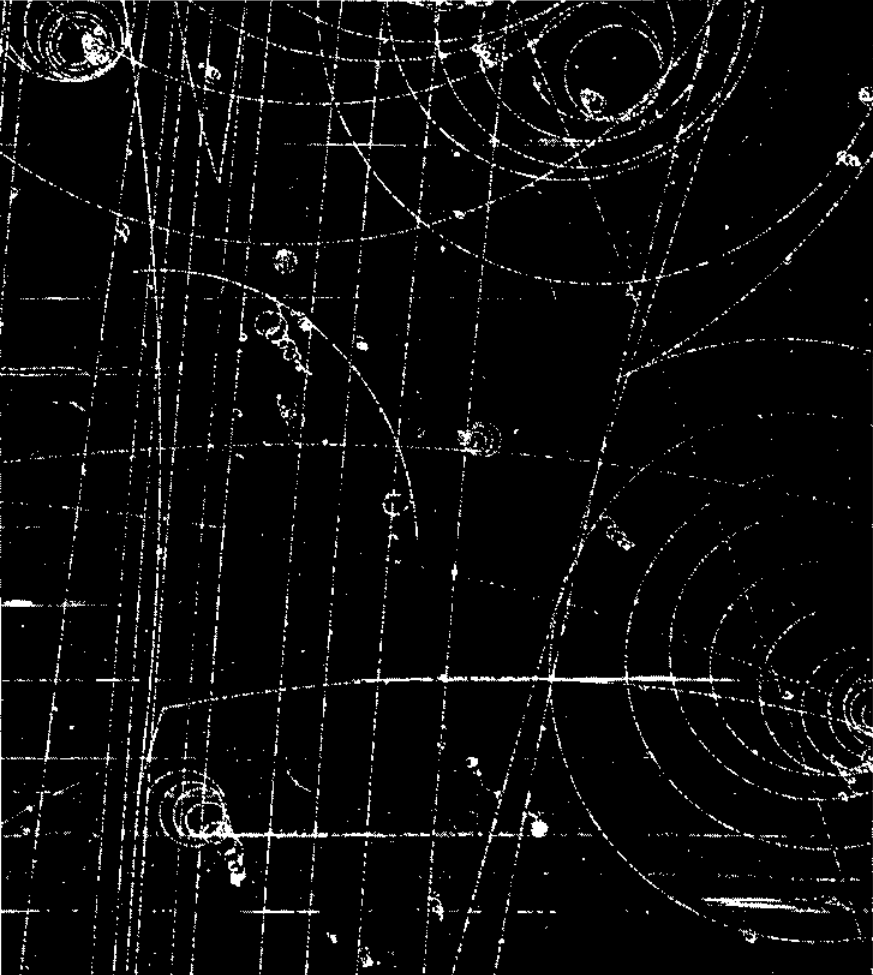
\includegraphics[width=\linewidth]{omega-minus-1.png}}\only<2->{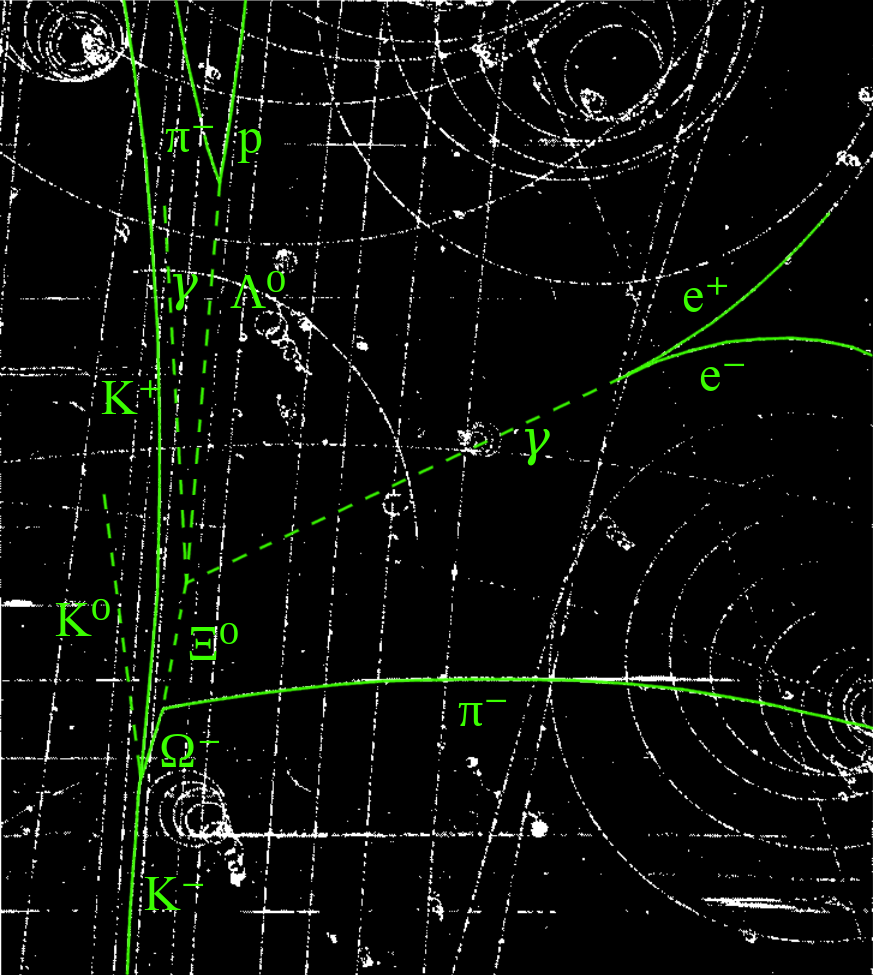
\includegraphics[width=\linewidth]{omega-minus-2.png}}
\column{0.5\linewidth}

\begin{center}
\begin{onlyenv}<1>
This is a famous photo: the 1964 discovery of the $\Omega$ baryon.

\vspace{1 cm}
Do you see it?

\vspace{1 cm}
\end{onlyenv}\begin{onlyenv}<2>
How about now?

\begin{align*}
K^- + p & \to \Omega^- \\
\Omega^- & \to \Xi^0 + \pi^- \\
\Xi^0 & \to \Lambda^0 + \gamma + \gamma \\
\Lambda^0 & \to p + \pi^-
\end{align*}

\vspace{1 cm}
\end{onlyenv}\begin{onlyenv}<3>
This is what particle physicists do: we collide particles, produce new ones and take pictures of their decay chains.

\vspace{1 cm}
However, these pictures come to us unlabeled: lots of interactions overlap the ``interesting'' ones.

\vspace{1 cm}
\end{onlyenv}
\end{center}

\end{columns}
\end{frame}

\begin{frame}{}
\begin{columns}
\column{1.15\linewidth}
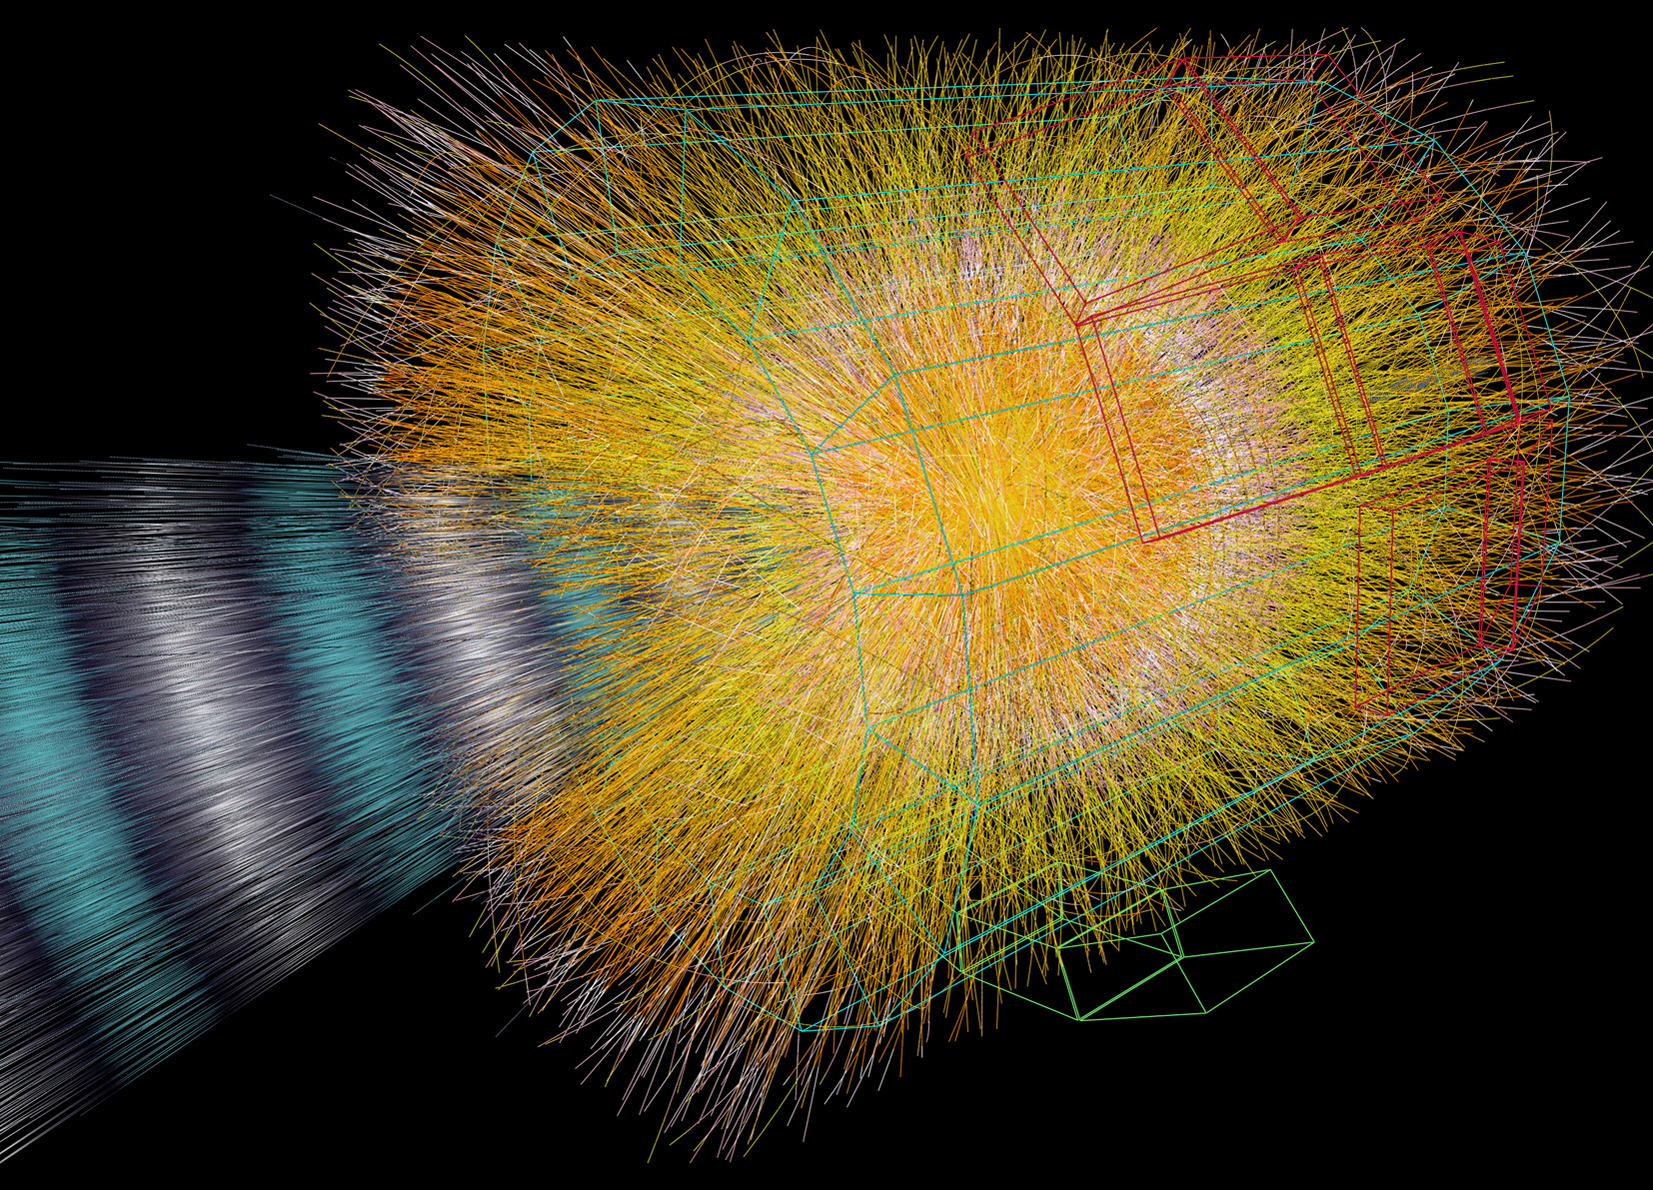
\includegraphics[width=\linewidth]{090324_ALICE-hirez.jpg}
\end{columns}
\end{frame}

\begin{frame}{Then and now}
\vspace{0.15 cm}
\begin{columns}
\column{0.32\linewidth}
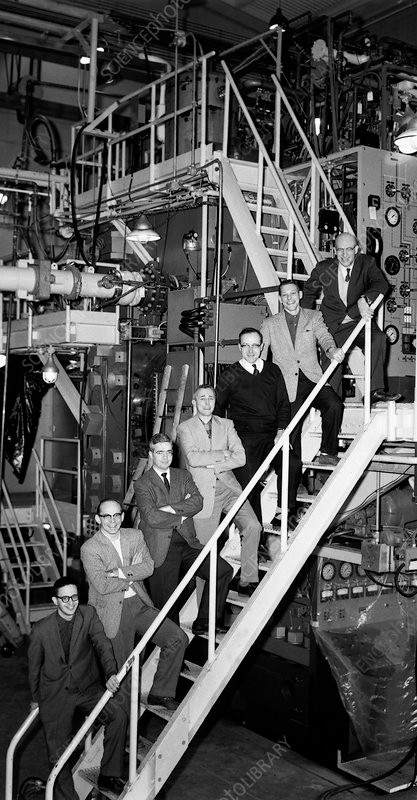
\includegraphics[width=\linewidth]{H4000010-Team_that_discovered_Omega_minus_particle.jpg}

\column{0.5\linewidth}
\begin{center}
\begin{columns}
\column{0.35\linewidth}
\centering
photographs

\vspace{0.5 cm}
100,000 events

\vspace{0.5 cm}
manual/semi-automated scans

\column{0.35\linewidth}
\centering
digitized signals \\

\vspace{0.5 cm}
$\sim$trillion events \\

\vspace{0.5 cm}
algorithmic searches and machine learning
\end{columns}
\end{center}

\column{0.32\linewidth}
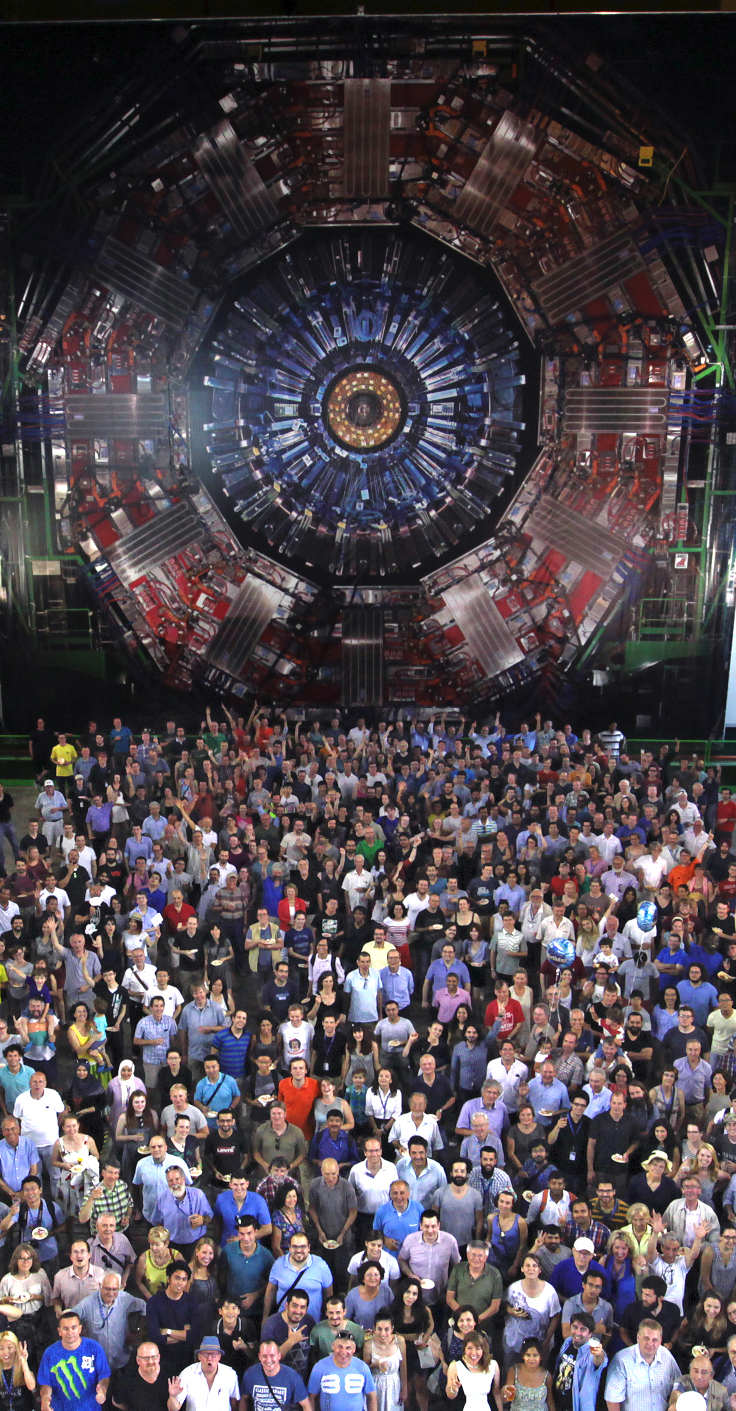
\includegraphics[width=\linewidth]{cms25_2.jpg}
\end{columns}
\end{frame}

\begin{frame}{}
\end{frame}

\end{document}
